\documentclass[11pt]{article}
\usepackage[margin=1in]{geometry}
\usepackage{amsmath,amssymb,graphicx,booktabs,hyperref,array,float}
\usepackage[T1]{fontenc}
\usepackage{lmodern}
\hypersetup{colorlinks=true,linkcolor=blue,citecolor=blue,urlcolor=blue}
\graphicspath{{figures/}}
\setlength{\emergencystretch}{2em}
\renewcommand{\topfraction}{.95}
\renewcommand{\bottomfraction}{.9}
\renewcommand{\textfraction}{.05}
\renewcommand{\floatpagefraction}{.8}
\setcounter{topnumber}{3}
\setcounter{totalnumber}{5}
\makeatletter
\setlength{\@fptop}{0pt}
\makeatother
\newcommand{\ForecastN}{706}
\newcommand{\OriginN}{10}
\newcommand{\CellN}{2300}
\newcommand{\ReleaseN}{23}
\newcommand{\GroupN}{71}
\newcommand{\IndustryN}{15}
\newcommand{\PairN}{1406}
\newcommand{\SubsetCandidates}{320}
\newcommand{\AbstractResult}{Industry models achieve the lowest aggregate MAE, 3.04 percentage points, compared with 3.39 for the six-release mean and 3.30 for the baseline. Nonlinear terms are repeatedly selected, but their subset model does not improve aggregate accuracy over the baseline.}
\newcommand{\ConclusionResult}{Industry-specific regression reduces aggregate MAE by 10.3\% relative to a six-release mean in this recorded sample. Elastic net and gradient boosting also improve accuracy. Nonlinear subset selection yields unstable functional forms and no aggregate improvement over the baseline. Overparameterized minimum-norm fits interpolate the training data and produce excessive future errors; regularization stabilizes this experiment.}

\title{Industry Heterogeneity and Nonlinear Forecasts of Small-Business AI Use}
\author{ISYE 4031: Group 1}
\date{October 26, 2026}
\begin{document}
\maketitle
\begin{abstract}
We examine industry differences in small-business artificial intelligence (AI) use and evaluate forecasts of published adoption rates three Census releases ahead. A reconstruction of the Business Trends and Outlook Survey reproduces the original Milestone 2 baseline. The extended analysis compares industry models, partial pooling, hierarchical subset selection with nonlinear terms, regularized regression, and gradient boosting under nested temporal validation. The evaluation comprises \ForecastN{} forecasts at \OriginN{} issue dates. \AbstractResult{}
Industry growth estimates are accompanied by uncertainty intervals and rank distributions. A controlled random-feature experiment evaluates prediction beyond the interpolation threshold. Selected AI release announcements are aligned with survey reference periods. The short observation window, informative missingness, and absence of an untreated comparison group restrict the interpretation of rankings and release-related changes.
\end{abstract}

\section{Introduction}
Small-business support organizations may use forecasts of AI adoption to anticipate demand for information, training, and implementation assistance. Such forecasts require evidence that improvements persist across industries, business sizes, and forecast dates. Differences in observed adoption also require uncertainty assessment: industries with similar estimated growth rates may have substantially overlapping rank distributions.

This study addresses three questions. First, do industry-specific relationships improve forecasts beyond a pooled linear baseline? Second, do quadratic terms and interactions provide predictive information after temporal validation? Third, how does forecast error change as the number of coefficients approaches and exceeds the number of training rows? We also examine the temporal correspondence between selected AI model releases and survey outcomes. The response is an industry-by-employment-size group's published AI-use percentage, rather than a firm-level adoption indicator or a measure of outreach effectiveness.

\section{Data and study population}
\subsection{Source and reconstruction}
The Census Business Trends and Outlook Survey (BTOS) publishes estimates for employer businesses. We restrict attention to five employment-size categories: 1--4, 5--9, 10--19, 20--49, and 50--99 employees. The comparable series begins with collection on November 17, 2025, when the AI question was broadened to cover any business function. Earlier observations are excluded because the wording change introduced a discontinuity \cite{wording}.

The original workbook was absent from the supplied project, and the Census download host returned timeouts during acquisition. The analysis therefore uses the unmodified, attributed CSV redistribution by The Uptime Report, which records a Census workbook extraction on October 15, 2026 \cite{extract}. The data include estimates, standard errors, collection dates, and national, industry, and size aggregates through release 202620. The file hash and acquisition record are supplied in the repository. This source reproduces the original report's historical cell counts and forecasting results; byte identity with the missing workbook cannot be established. Other business-condition survey questions are unavailable in the extract and do not enter the reported fits.

The original historical window contains 22 releases through 202619: 2,200 potential cells and 498 unavailable current-use estimates. The reconstructed analysis adds release 202620, giving \CellN{} potential cells across \ReleaseN{} releases. Missing rows in the extract are treated as unavailable values. Their individual original suppression flags cannot be recovered. BTOS withholds estimates for quality or disclosure concerns, including relative standard errors above 50\% \cite{censusmethods}. Missing current-use rates and forecast outcomes are never imputed.

\subsection{Screening and temporal alignment}
A group is retained when both current and expected AI use are published in at least seven of the first eight releases. Multi-sector category XX is excluded. The rule retains \GroupN{} groups in \IndustryN{} industries and is applied before the first evaluation date. The resulting population consists of relatively well-measured industry-size groups. It does not represent all small businesses, and group-level averages are not business-population-weighted averages.

Let $y_{g,t}$ denote the current-use percentage for group $g$ at release $t$, and let $e_{g,t}$ denote expected use over the next six months. We predict $y_{g,t+3}$ at the publication of release $t$. Three releases correspond to approximately six weeks. Reference periods, collection periods, and publication dates are distinct. For the included extract, publication is reconstructed as the Thursday following collection; this schedule reproduces the original report's forecast dates. Event analyses use the previous fortnight's reference period, with its end one day before collection begins. The calendar is exported for inspection.

There are \PairN{} complete issue--target pairs in the extended sample. Historical evaluation covers the original nine issue dates; the extension contains one additional issue date. All expanded specifications were developed after the extension outcome was publicly available. Consequently, the extension is a retrospective temporal test of these specifications, rather than a newly conducted prospective experiment.

\section{Statistical methods}
\subsection{Forecast models}
The original baseline is pooled ordinary least squares (OLS):
\begin{equation}
 y_{g,t+3}=\beta_0+\beta_y y_{g,t}+\alpha_{s(g)}+\delta_{b(g)}+\beta_t t+\varepsilon_{g,t+3},
\end{equation}
where $s(g)$ and $b(g)$ identify industry and size. Benchmarks carry forward the latest rate or average the latest six available releases. Separate industry regressions allow each industry's coefficients to differ. A partial-pooling estimator retains unpenalized global intercept, current-use, and time coefficients, while ridge penalties shrink industry and size intercept deviations and industry trend deviations. This estimator is a penalized regression; it is not a fitted random-effects likelihood.

The full feature dictionary includes current and expected use, linear time, squared current use, squared expected use, squared time, current-use-by-time and current-by-expected-use products, industry-specific current-use slopes and trends, size-specific trends, lags of 1, 2, 3, and 6 releases, a six-release average, recent change, the expectation gap, the current estimate's standard error, and available national, industry, and size AI-use and expectation aggregates. It also includes a known sample-year indicator and sine/cosine terms with period six releases. The latter investigate the rotating-panel cycle; the available history cannot establish annual seasonality. Supplementary missing predictors are median-imputed using training rows only, with missingness indicators. Numerical features are standardized within each training fold.

We compare full OLS, ridge regression, elastic net, and histogram gradient boosting. Ridge penalties are selected from $\{0.1,1,10,100,1000,10000,100000\}$. Elastic net uses a mixing fraction of $0.5$ and penalties $\{0.01,0.1,0.5,1\}$. Boosting uses 150 iterations, learning rate $0.05$, at least 25 observations per leaf, an $L_2$ penalty of 10, and maximum leaf counts $\{3,7,15\}$. These finite dictionaries constrain the search in a short panel.

\subsection{Hierarchical subset selection and nonlinearity}
Subset selection retains the baseline's main effects and exhaustively searches optional blocks. A linear comparison permits expected use and industry- or size-specific slopes and trends. The nonlinear search additionally permits $y^2$, $e^2$, $t^2$, $yt$, and $ye$. Industry indicators and their interactions enter as blocks. Strong hierarchy requires the expected-use main effect whenever $e^2$ or $ye$ is selected; the remaining parent effects are already mandatory. Each of the \SubsetCandidates{} admissible nonlinear candidates is fitted by least squares. Selection minimizes average validation-origin MAE; exact ties favor fewer columns. This is best subset selection over a specified block dictionary, rather than exhaustive selection over every derived predictor \cite{subset}.

A quadratic term or interaction remains linear in its fitted coefficient while allowing nonlinear or industry-dependent response relationships. Its selection is evidence of predictive utility within the candidate dictionary. Selection frequencies across outer origins measure stability. Conventional coefficient tests performed after searching would omit selection uncertainty, so we do not interpret selected-term $p$-values as confirmatory evidence.

\subsection{Nested temporal evaluation}
At an outer issue date $d_t$, the training sample satisfies
\begin{equation}
 \mathcal{T}_t=\{(g,u):\operatorname{publication}(u+3)\le d_t\}.
\end{equation}
The outer test consists of complete pairs issued at $t$. Within $\mathcal{T}_t$, up to four earlier validation origins span the available history. Each inner fit again excludes targets unpublished at its own issue date. Subset choice, regularization, and boosting complexity use only these inner predictions. Screening, preprocessing, and selection therefore do not use outer outcomes. Historical data vintages cannot be reconstructed from the redistributed file, so this is temporal validation of the recorded vintage rather than a complete real-time vintage experiment.

Forecast accuracy is evaluated by mean absolute error (MAE), root mean squared error (RMSE), and bias, all in percentage points (pp), with industry and size breakdowns. Predictions are not clipped to $[0,100]$; the frequency of violations is recorded. Paired differences in origin-level MAE are summarized with 2,000 circular moving-block bootstrap draws of length three origins. These intervals address dependence across nearby forecasts approximately. With only \OriginN{} origins they remain exploratory. Exact sign-flip calculations are supplied as a sensitivity calculation under an exchangeability assumption; they are not relied upon for inference under serial dependence. Comparisons across several models introduce additional selection uncertainty.

Survey standard errors quantify uncertainty in the published target. We report their relationship to forecast errors without treating them as a strict lower bound on MAE. Sampling error, temporal dependence, model error, and uncertainty about the underlying adoption rate are distinct quantities.

\subsection{Industry growth and ranking uncertainty}
For descriptive industry growth, we fit
\begin{equation}
 y_{g,t}=a_g+\gamma_{s(g)}(t/2)+u_{g,t},
\end{equation}
with group intercepts $a_g$. The coefficient $\gamma_s$ is the change in percentage points per four weeks, using two releases per four weeks. Equal observation weights define the primary estimand; retained size bands need not be identical across industries.

Uncertainty is estimated with 2,000 wild residual bootstrap draws. Six-release blocks share multipliers across all groups, and block boundaries have random offsets. This retains common release shocks and approximates within-cycle dependence. We report percentile intervals, median ranks, rank ranges, and the proportion of bootstrap draws placing an industry in the top three. These proportions describe resampling stability, not posterior probabilities. The small number of temporal blocks and residual-model assumptions restrict precision. Pairwise difference intervals are exploratory and are not simultaneous confidence intervals. Sensitivity fits add a common indicator at release 202616, when the annual sample changes, or weight observations inversely by the squared published standard error with a 1-pp standard-error floor.

\subsection{Model-release timing}
Six provider announcements form a selected chronology: Gemini 3, Claude Opus 4.5, GPT-5.2, Claude Opus 4.6, Gemini 3.1 Pro, and GPT-5.4 \cite{gemini3,opus45,gpt52,opus46,gemini31,gpt54}. For each event, we compare three complete reference fortnights before the announcement with three wholly subsequent fortnights, excluding a straddling window. Events without three pre- and post-event observations are marked unsupported. A constant set of groups with observed rates at every release prevents changing suppression patterns from mechanically shifting the aggregate.

We also regress the balanced-group mean on time, a sample-change indicator, and the cumulative number of selected announcements. Releases overlap in time and exposure is common to all industries. The resulting coefficient is descriptive: adoption trends, survey changes, and other contemporaneous events supply alternative explanations. The design does not identify an announcement's causal effect.

\subsection{Overparameterization experiment}
To vary parameter count while holding input information fixed, we transform standardized baseline and expected-use inputs into nested random Fourier features,
\begin{equation}
 z_j(x)=\sqrt{2/m}\cos(\omega_j^{\mathsf T}x+b_j),\quad
 \omega_j\sim N(0,I/d),\quad b_j\sim U(0,2\pi),
\end{equation}
where $d$ is input dimension. Feature centering uses training rows. Three seeds and the first, middle, and final outer origins are evaluated at coefficient-to-row ratios near $0.05$, $0.2$, $0.5$, $0.8$, $1$, $1.2$, and $2$. All widths use the same initial feature sequence within a seed. The intercept is included in coefficient counts and matrix rank.

For each width we fit minimum-norm least squares and ridge regression with fixed penalty $0.01$. The ridge objective uses the unnormalized residual sum of squares, and the penalty is fixed as a diagnostic rather than tuned on test outcomes. We record rank, effective degrees of freedom, condition number, and training and future errors. Numerical interpolation is assessed directly. Increasing $p$ beyond $n$ does not by itself establish interpolation when the matrix is rank deficient. A fall in future error after a peak near interpolation would be consistent with double descent \cite{belkin}; its occurrence is evaluated empirically for this feature family.

\section{Results}
\subsection{Forecast accuracy and industry heterogeneity}
Table~\ref{tab:performance} reports all forecast specifications on a common evaluation sample. Separate industry models have the lowest aggregate MAE, 3.04 pp, compared with 3.39 for the six-release mean and 3.30 for the original pooled baseline. These differences correspond to reductions of 10.3\% and 8.0\%, respectively. Elastic net (3.07), gradient boosting (3.12), and ridge (3.13) also improve on the recent-average benchmark. Partial pooling yields 3.29 pp, close to the baseline. The full unregularized dictionary yields MAE of 5.68 pp and produces six predictions outside the percentage range.

\begin{table}[!htbp]
\centering
\small
\caption{Forecast errors in percentage points. Historical: 635 forecasts at nine origins; extension: 71 forecasts at one origin; all: 706 forecasts.}\label{tab:performance}
\begin{tabular}{lrrrrr}
\toprule
Model & Historical MAE & Extension MAE & All MAE & All RMSE & All bias \\
\midrule
Persistence & 4.18 & 3.90 & 4.15 & 5.75 & -1.05 \\
Six-release mean & 3.40 & 3.34 & 3.39 & 4.64 & -2.07 \\
Baseline OLS & 3.33 & 3.09 & 3.30 & 4.55 & +0.07 \\
Linear subset & 3.39 & 3.06 & 3.36 & 4.63 & +0.03 \\
Nonlinear subset & 3.36 & 2.97 & 3.32 & 4.66 & +0.12 \\
Full OLS & 5.92 & 3.52 & 5.68 & 7.27 & +2.11 \\
Ridge & 3.15 & 2.99 & 3.13 & 4.32 & +0.47 \\
Elastic net & 3.08 & 2.93 & 3.07 & 4.29 & +0.06 \\
Gradient boosting & 3.12 & 3.09 & 3.12 & 4.38 & -0.03 \\
Partial pooling & 3.33 & 2.97 & 3.29 & 4.51 & +0.12 \\
Industry models & 3.04 & 3.02 & 3.04 & 4.29 & -0.21 \\
\bottomrule
\end{tabular}
\end{table}


Industry models beat the recent mean at nine of ten issue dates. Their mean origin-level difference is $-0.35$ pp, with exploratory block interval $[-0.46,-0.24]$. Relative to baseline OLS, the corresponding difference is $-0.26$ pp, with interval $[-0.40,-0.12]$. Ridge and boosting beat the recent mean at all ten dates. These results support industry heterogeneity and regularization within this sample, although the short evaluation history limits claims about future performance.

\begin{table}[!htbp]
\centering
\small
\caption{Paired origin-level MAE differences relative to the six-release mean. Negative values favor the fitted model. Intervals are 95\% moving-block bootstrap intervals and are exploratory.}\label{tab:paired}
\begin{tabular}{lrrr}
\toprule
Model & Difference (pp) & Interval (pp) & Origins won \\
\midrule
Baseline OLS & -0.09 & [-0.22, +0.04] & 7/10 \\
Linear subset & -0.03 & [-0.15, +0.10] & 4/10 \\
Nonlinear subset & -0.07 & [-0.20, +0.08] & 6/10 \\
Full OLS & +2.29 & [+0.71, +3.91] & 1/10 \\
Ridge & -0.25 & [-0.36, -0.17] & 10/10 \\
Elastic net & -0.32 & [-0.43, -0.21] & 9/10 \\
Gradient boosting & -0.27 & [-0.45, -0.13] & 10/10 \\
Partial pooling & -0.10 & [-0.23, +0.05] & 5/10 \\
Industry models & -0.35 & [-0.46, -0.24] & 9/10 \\
\bottomrule
\end{tabular}
\end{table}


\begin{figure}[htbp]
\centering
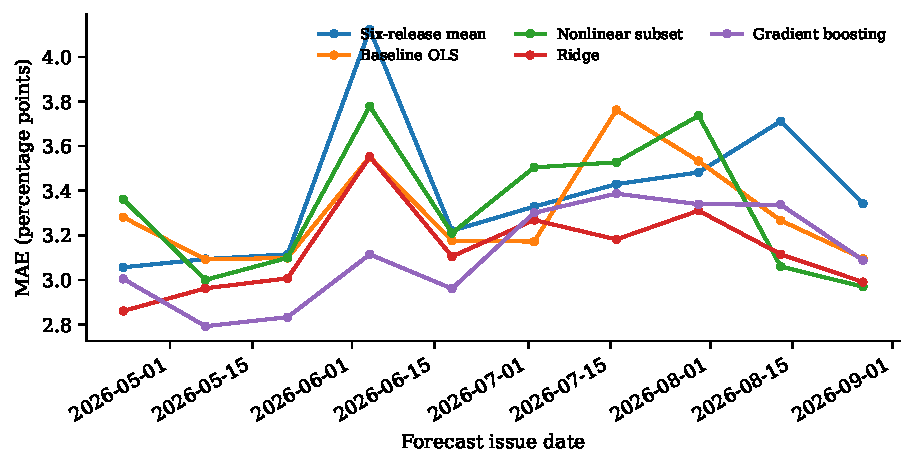
\includegraphics[width=.95\linewidth]{errors_by_origin.pdf}
\caption{Forecast MAE by issue date. All lines use identical evaluated group-release pairs. The final point forecasts the extension outcome.}
\label{fig:origins}
\end{figure}

Industry models reduce MAE for the 50--99 employee band from 5.32 pp under the baseline to 4.23 pp, below the recent mean's 4.65 pp. The advantage is not uniform: for the 10--19 employee band, ridge and elastic net perform better than separate industry models. At the industry level, Information remains difficult: its industry-model MAE is 6.48 pp. Aggregate improvement therefore does not justify equally confident forecasts for every group. The median published target standard error is 2.83 pp; 88.8\% of industry-model errors fall within twice the corresponding target standard error. This comparison describes the scale of survey uncertainty and does not establish interval calibration.

The extension contains one origin and cannot establish general superiority. Elastic net has its lowest extension MAE at 2.93 pp, followed by nonlinear subset selection at 2.97 pp. Industry models achieve 3.02 pp, compared with 3.09 for the baseline and 3.34 for the recent mean. All expanded methods remain retrospectively specified.

\subsection{Selected nonlinear structure}
The nonlinear search selects an industry-by-current-use interaction at every outer origin. Expected use squared and the current-use-by-time interaction are selected at six of ten origins; the current-by-expected-use interaction appears at the other four. Current use squared and time squared are never selected. Thus the candidate search finds industry-dependent slopes and some curvature in expectations, without evidence that a quadratic current-use response is consistently needed.

The nonlinear subset achieves aggregate MAE of 3.32 pp, compared with 3.36 for the linear subset and 3.30 for the baseline. Its mean origin-level improvement over the linear subset is only 0.03 pp, with interval $[-0.068,0.005]$ for the nonlinear-minus-linear difference. Relative to the baseline, its difference is $+0.02$ pp with interval $[-0.064,0.120]$. These comparisons provide limited support for an incremental predictive benefit from the nonlinear terms.

\begin{figure}[htbp]
\centering
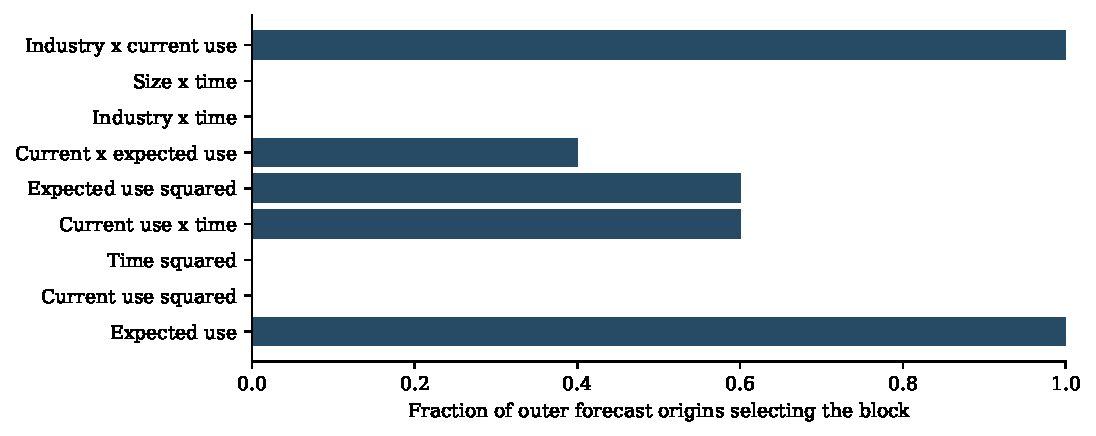
\includegraphics[width=.95\linewidth]{subset_stability.pdf}
\caption{Selection frequency of optional blocks. Main effects for current use, time, industry, and size are mandatory. An interaction with industry allows slopes to differ across sectors.}
\label{fig:selection}
\end{figure}

\begin{figure}[htbp]
\centering
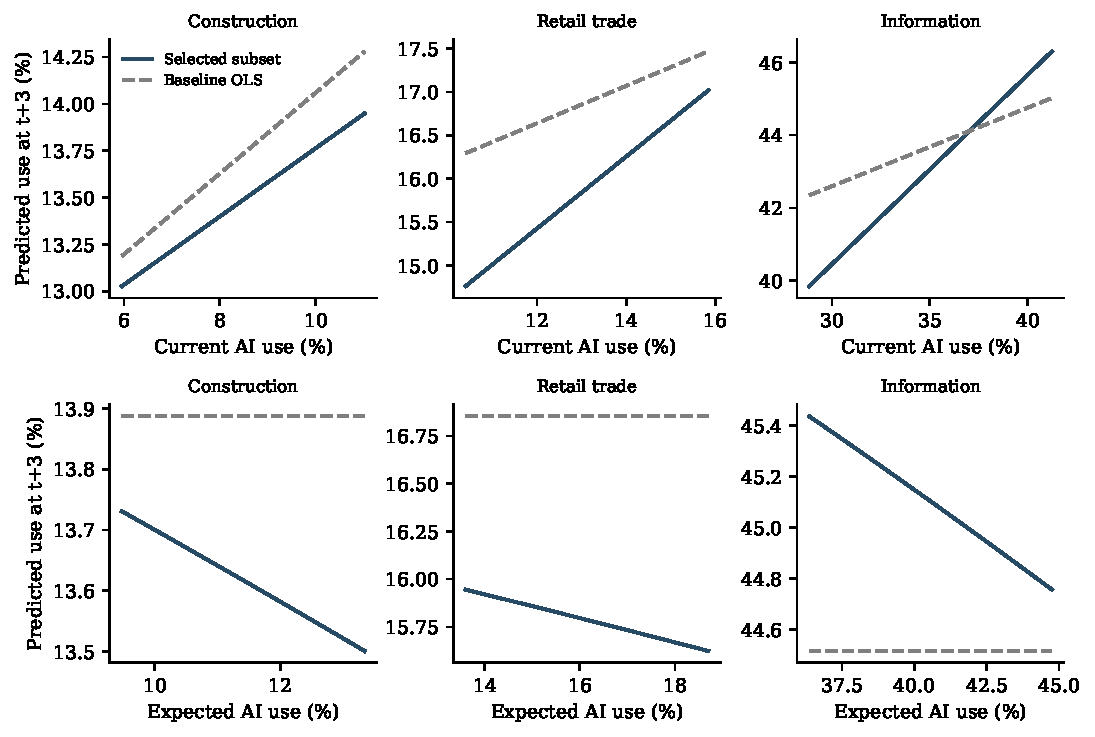
\includegraphics[width=.97\linewidth]{conditional_curves.pdf}
\caption{Conditional predictions from the final nonlinear subset and baseline, for 1--4 employee firms in three industries. The varying predictor spans its within-group training 5th--95th percentiles. The other adoption predictor is fixed at its within-group training median, and time is fixed at the final issue date. The final subset includes expected use squared; its current-use relationship is linear when time and expectations are held fixed. These curves describe fitted relationships without causal interpretation.}
\label{fig:curves}
\end{figure}

Ridge ablations reinforce the importance of recent history. Removing lagged rates, recent change, and the rolling mean increases MAE from 3.13 to 3.70 pp. Removing the six-release cycle changes MAE only to 3.15 pp. Removing quantitative curvature terms gives 3.12 pp, and omitting contemporaneous aggregate rates also gives 3.12 pp. These small latter differences do not establish useful seasonality or a material gain from the larger dictionary. The ridge search selects penalty 1,000 at all origins, even after expanding the grid to 100,000.

\subsection{Industry growth and ranking}
Finance and insurance has the highest estimated growth, 1.28 pp per four weeks, followed by Information at 1.22 and professional and technical services at 1.08. Their conditional intervals are $[1.07,1.48]$, $[0.95,1.50]$, and $[0.94,1.21]$, respectively. Accommodation and food services grows by 0.16 pp per four weeks, with interval $[0.11,0.21]$. All retained industries have positive fitted trends in the observed period. These are absolute percentage-point changes; rankings by relative percentage growth would answer a different question.

\begin{figure}[htbp]
\centering
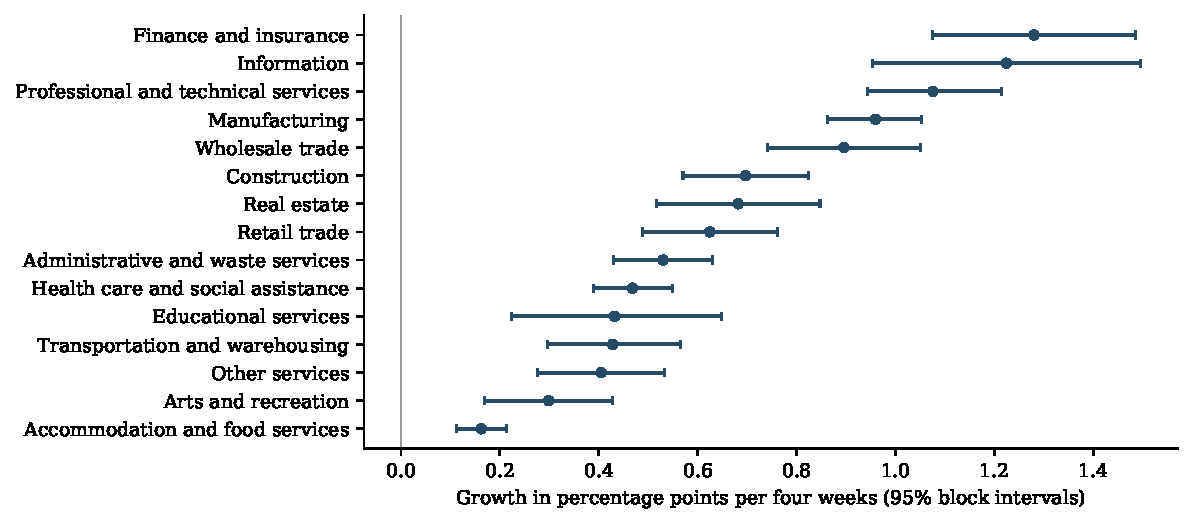
\includegraphics[width=.96\linewidth]{industry_growth.pdf}
\caption{Industry-specific growth with conditional 95\% wild block bootstrap intervals. Group intercepts account for stable industry-size differences. Results apply to retained size groups and are not population-weighted industry estimates.}
\label{fig:growth}
\end{figure}

The top two industries cannot be confidently ordered. The Information-minus-finance growth difference is $-0.06$ pp per four weeks, with interval $[-0.38,0.27]$. Finance has a bootstrap rank range of 1--3, Information 1--4, and professional services 2--3. Finance, Information, and professional services occupy the top three in 100.0\%, 97.2\%, and 97.8\% of bootstrap draws, respectively. These frequencies are conditional on the fitted trend model and a short series. They support a leading group more strongly than a precise ordering within that group.

\begin{figure}[htbp]
\centering
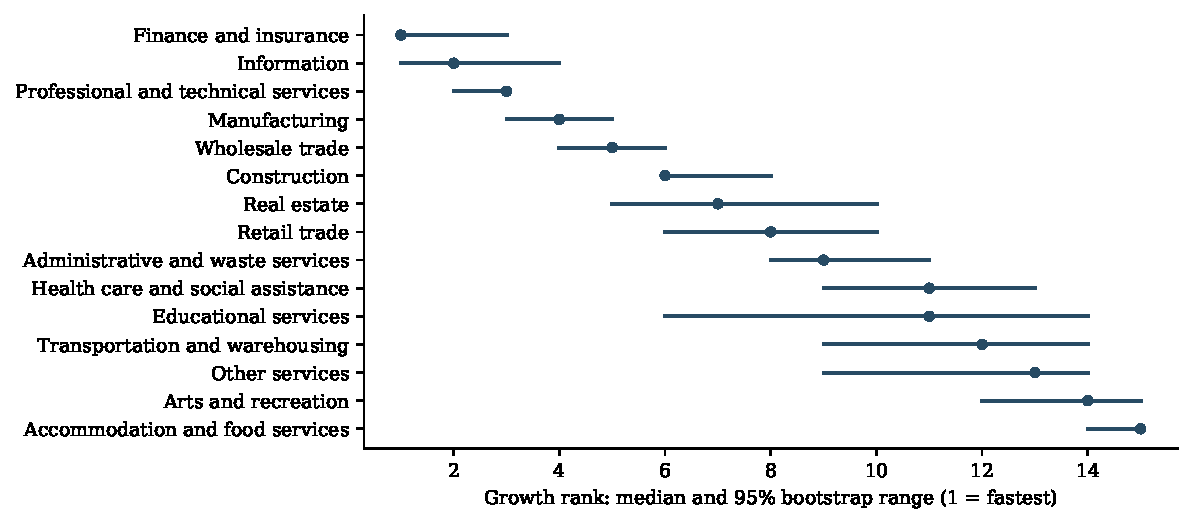
\includegraphics[width=.96\linewidth]{industry_ranks.pdf}
\caption{Median growth ranks and central 95\% bootstrap rank ranges. Overlapping ranges indicate uncertainty in exact ordering; the ranges are not simultaneous confidence sets.}
\label{fig:ranks}
\end{figure}

Adding a common sample-change indicator preserves the primary ordering closely. Inverse-variance weighting changes the relative ordering of the top two: Information's estimated growth becomes 1.16 pp per four weeks and finance's 1.14. This sensitivity is consistent with their overlapping uncertainty. The leading group remains substantively similar.

\subsection{Release chronology}
The event analysis uses 65 groups with observed rates at all 23 releases. The three earliest announcements have fewer than three pre-event reference periods in the comparable series and cannot support the specified window comparison. For the February and March events with sufficient observations, three-period pre/post changes are positive: 0.45 pp for Claude Opus 4.6, 1.43 pp for Gemini 3.1 Pro, and 1.61 pp for GPT-5.4. The reference windows overlap substantially.

\begin{figure}[htbp]
\centering
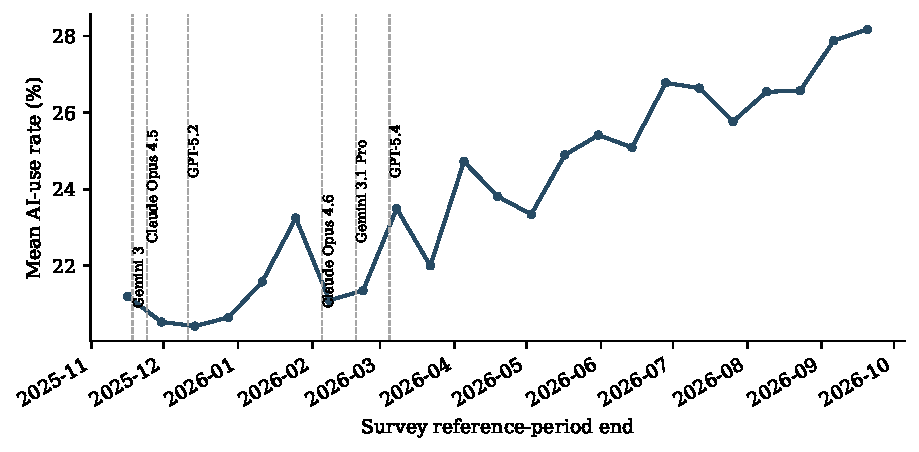
\includegraphics[width=.95\linewidth]{release_timeline.pdf}
\caption{Balanced-group AI-use mean by reference-period end, with selected provider announcement dates. Publication occurs after the reference period and collection. Event positions indicate temporal correspondence; the figure does not estimate causal effects.}
\label{fig:events}
\end{figure}

The cumulative announcement count correlates 0.81 with time. After adjustment for a linear trend and the sample-change indicator, its descriptive coefficient is $-0.47$ pp per selected announcement. This sign differs from the positive unadjusted window changes. The contrast illustrates sensitivity to trend adjustment and the limited independent information in a common event chronology. It does not establish a negative effect of model releases. The data do not separate release effects from ongoing diffusion or other calendar-time influences.

\subsection{Interpolation and overparameterization}
The random-feature design reaches full row rank, including the intercept, near $p/n=1$. Minimum-norm training error approaches zero there. Median future RMSE rises from 5.63 pp at $p/n=0.2$ to approximately 4,577 pp at interpolation. It then falls to approximately 190 pp at $p/n=1.2$, remaining near 203 pp at $p/n=2$. This post-peak reduction is a second-descent pattern over part of the tested range, but its prediction errors remain far above those of the practical forecasting models.

\begin{figure}[htbp]
\centering
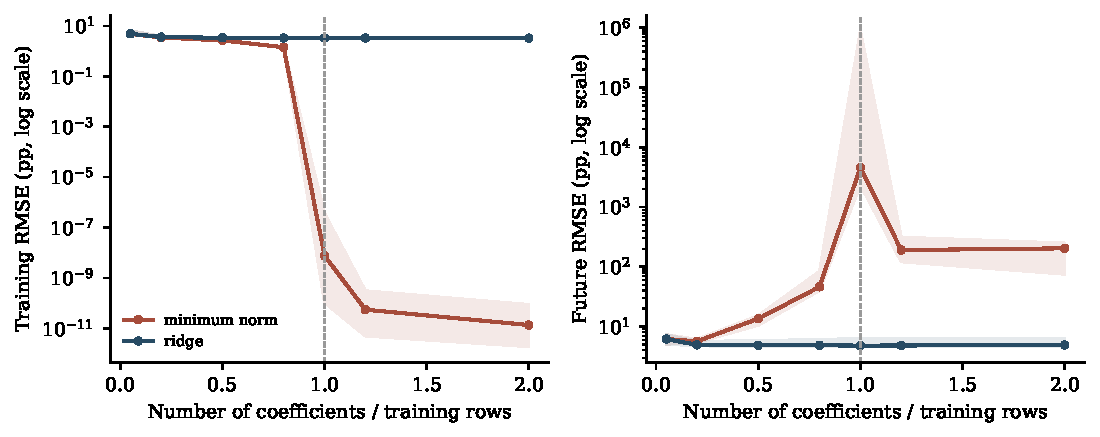
\includegraphics[width=\linewidth]{complexity.pdf}
\caption{Training and future RMSE across model widths, using logarithmic error axes. Lines show medians over three origins and three feature seeds; shading shows the 10th--90th percentiles across those nine fits, rather than confidence intervals. The vertical line marks $p/n=1$. Ridge uses a fixed diagnostic penalty of 0.01.}
\label{fig:complexity}
\end{figure}

Ridge avoids interpolation and keeps median future RMSE near 4.77--4.89 pp for $p/n$ between 1 and 2. At $p/n=2$, its median effective degrees of freedom are approximately 210, compared with a median training-row count of 912. Thus a nominally overparameterized representation can remain strongly regularized. This experiment establishes the existence of interpolating fits in the chosen representation, while providing no evidence that unregularized overparameterization improves useful forecasting performance.

The practical full OLS model already performs poorly with 81 nominal coefficients and training samples of 560--1,195 rows. Its recorded ranks are 78--80 because the dictionary includes redundant relationships. Predictive instability therefore arises well before the formal $p>n$ regime.


\section{Discussion}
The clearest forecasting result is the value of allowing industries to differ. Separate industry regressions reduce average error relative to the original pooled specification and improve the previously weak 50--99 employee band. Regularized pooled models also improve performance. The unrestricted full dictionary performs substantially worse, and removing quantitative curvature from ridge has little effect. These findings favor targeted heterogeneity, historical smoothing, and coefficient control over indiscriminate expansion of the regression equation.

Nonlinear subset selection identifies industry-dependent slopes and a curved association between expectations and future published use. The selected expectation form changes across validation dates and does not deliver an aggregate improvement over the baseline. The final subset gives a decreasing conditional relationship with expected use over the plotted ranges, further limiting a structural interpretation. The statistical conclusion is therefore limited: the candidate dictionary contains nonlinear descriptions, but their incremental predictive value has not been established. A subsequent preregistered comparison on genuinely future releases would provide stronger evidence.

For industry comparisons, finance, Information, and professional services form a relatively stable leading growth group. Their exact ordering is uncertain. Outreach organizations could use these results to distinguish broad adoption trajectories while avoiding precise league tables. Higher adoption or faster growth does not establish unmet need, accessibility of assistance, or the benefit of an intervention. Resource-allocation decisions require additional information on barriers, costs, and program outcomes.

The interpretation of uncertainty remains conditional. Estimates arise from a short, noisy panel with recurring groups, shared date shocks, and a rotating business sample. The six-release block bootstrap has few effective temporal blocks. It is not a substitute for Census replicate weights or full design-based covariance information. Standard errors address sampling variability, while nonresponse and interpretation changes can introduce additional error. Screening excludes groups with frequent missing estimates, and the results may not transfer to those groups. Equal weighting across retained cells also differs from weighting industries by their business populations.

The event study supplies a useful chronology but cannot attribute adoption changes to specific releases. Announcements are common exposures, cluster early in the sample, and overlap with a strong adoption trend. Early releases lack comparable pre-event data. A stronger design would link firm or industry exposure to particular tools, specify comparison groups before inspecting outcomes, and assess pre-event trends over a longer consistent series.

Finally, the capacity experiment shows why parameter count alone is an inadequate guide to forecasting. Minimum-norm interpolation produces extreme errors in this noisy setting, although error declines after the interpolation peak. Ridge stabilizes a much larger feature representation through shrinkage. These results are specific to the tested random-feature distribution, fixed bandwidth, penalty, origins, and seeds; they do not establish a universal double-descent curve for BTOS or for machine learning generally.


\section{Conclusion}
\ConclusionResult{}
The practical value of a forecast depends on stable performance across issue dates and relevant business groups. Ranking uncertainty should accompany industry comparisons. Release timing provides hypotheses for further investigation, while credible causal attribution would require additional exposure information or an appropriate comparison design.

\section*{Acknowledgments}
AI assistance was used to develop the analysis code and revise the manuscript. The original Milestone 2 report and scripts are preserved in the repository.

\begin{thebibliography}{99}
\small\raggedright
\bibitem{censusmethods} U.S. Census Bureau. \emph{Business Trends and Outlook Survey Methodology}, Version 5, October 2026. \url{https://www2.census.gov/data/experimental-data-products/business-trends-and-outlook-survey/methodology.pdf}.
\bibitem{wording} U.S. Census Bureau. \emph{BTOS AI Core Question Updates}, December 3, 2025. \url{https://www.census.gov/hfp/btos/downloads/AI%20Question%20Wording%20Updates.pdf}.
\bibitem{extract} The Uptime Report. \emph{Small Business AI Adoption: Census BTOS Data}, October 2026. Census estimates redistributed under CC BY 4.0; workbook extraction dated October 15, 2026. \url{https://theuptimereport.com/small-business-ai-adoption/}.
\bibitem{subset} Stanford University. \emph{STATS 202: Stepwise Selection Methods}. \url{https://web.stanford.edu/class/stats202/notes/Model-selection/Stepwise.html}.
\bibitem{belkin} Belkin, M., Hsu, D., Ma, S., and Mandal, S. (2019). Reconciling modern machine-learning practice and the classical bias--variance trade-off. \emph{Proceedings of the National Academy of Sciences}, 116, 15849--15854. \url{https://doi.org/10.1073/pnas.1903070116}.
\bibitem{gemini3} Google. \emph{Gemini 3 Brings Upgraded Smarts and New Capabilities to the Gemini App}, November 18, 2025. \url{https://blog.google/products-and-platforms/products/gemini/gemini-3-gemini-app/}.
\bibitem{opus45} Anthropic. \emph{Introducing Claude Opus 4.5}, November 24, 2025. \url{https://www.anthropic.com/news/claude-opus-4-5}.
\bibitem{gpt52} OpenAI. \emph{Introducing GPT-5.2}, December 11, 2025. \url{https://openai.com/index/introducing-gpt-5-2/}.
\bibitem{opus46} Anthropic. \emph{Introducing Claude Opus 4.6}, February 5, 2026. \url{https://www.anthropic.com/news/claude-opus-4-6}.
\bibitem{gemini31} Google DeepMind. \emph{Gemini 3.1 Pro Model Card}, February 19, 2026. \url{https://deepmind.google/models/model-cards/gemini-3-1-pro}.
\bibitem{gpt54} OpenAI. \emph{Introducing GPT-5.4}, March 5, 2026. \url{https://openai.com/index/introducing-gpt-5-4/}.
\end{thebibliography}
\clearpage
\appendix
\section{Additional results and reproducibility}
\begin{table}[H]
\centering
\small
\caption{Industry growth in percentage points per four weeks. Intervals and rank ranges summarize the conditional wild block bootstrap; top-three shares are resampling frequencies.}\label{tab:growth}
\begin{tabular}{lrrrr}
\toprule
Industry & Growth & 95\% interval & Rank range & Top three \\
\midrule
Finance and insurance & 1.28 & [1.07, 1.48] & 1--3 & 100.0\% \\
Information & 1.22 & [0.95, 1.50] & 1--4 & 97.2\% \\
Professional and technical services & 1.08 & [0.94, 1.21] & 2--3 & 97.8\% \\
Manufacturing & 0.96 & [0.86, 1.05] & 3--5 & 3.8\% \\
Wholesale trade & 0.90 & [0.74, 1.05] & 4--6 & 1.3\% \\
Construction & 0.70 & [0.57, 0.82] & 6--8 & 0.0\% \\
Real estate & 0.68 & [0.52, 0.85] & 5--10 & 0.0\% \\
Retail trade & 0.62 & [0.49, 0.76] & 6--10 & 0.0\% \\
Administrative and waste services & 0.53 & [0.43, 0.63] & 8--11 & 0.0\% \\
Health care and social assistance & 0.47 & [0.39, 0.55] & 9--13 & 0.0\% \\
Educational services & 0.43 & [0.22, 0.65] & 6--14 & 0.0\% \\
Transportation and warehousing & 0.43 & [0.30, 0.57] & 9--14 & 0.0\% \\
Other services & 0.40 & [0.28, 0.53] & 9--14 & 0.0\% \\
Arts and recreation & 0.30 & [0.17, 0.43] & 12--15 & 0.0\% \\
Accommodation and food services & 0.16 & [0.11, 0.21] & 14--15 & 0.0\% \\
\bottomrule
\end{tabular}
\end{table}

\begin{table}[H]
\centering
\small
\caption{Sensitivity of growth estimates (pp per four weeks) to a common sample-change indicator and inverse-variance weighting. Primary confidence intervals do not apply to these sensitivity fits.}\label{tab:sensitivity}
\begin{tabular}{lrrr}
\toprule
Industry & Primary & Sample adjusted & SE weighted \\
\midrule
Finance and insurance & 1.28 & 1.29 & 1.14 \\
Information & 1.22 & 1.24 & 1.16 \\
Professional and technical services & 1.08 & 1.09 & 0.96 \\
Manufacturing & 0.96 & 0.97 & 0.87 \\
Wholesale trade & 0.90 & 0.91 & 0.76 \\
Construction & 0.70 & 0.71 & 0.72 \\
Real estate & 0.68 & 0.70 & 0.65 \\
Retail trade & 0.62 & 0.64 & 0.45 \\
Administrative and waste services & 0.53 & 0.54 & 0.52 \\
Health care and social assistance & 0.47 & 0.48 & 0.55 \\
Educational services & 0.43 & 0.45 & 0.50 \\
Transportation and warehousing & 0.43 & 0.44 & 0.40 \\
Other services & 0.40 & 0.42 & 0.36 \\
Arts and recreation & 0.30 & 0.31 & 0.15 \\
Accommodation and food services & 0.16 & 0.18 & 0.17 \\
\bottomrule
\end{tabular}
\end{table}

\begin{table}[H]
\centering
\small
\caption{Nonlinear-subset selection frequency over ten outer origins. Baseline main effects are mandatory.}\label{tab:selection}
\begin{tabular}{lrr}
\toprule
Optional block & Selected origins & Frequency \\
\midrule
Expected use & 10 & 100\% \\
Current use squared ($y_t^2$) & 0 & 0\% \\
Time squared ($t^2$) & 0 & 0\% \\
Current use $\times$ time & 6 & 60\% \\
Expected use squared ($e_t^2$) & 6 & 60\% \\
Current $\times$ expected use & 4 & 40\% \\
Industry $\times$ time & 0 & 0\% \\
Size $\times$ time & 0 & 0\% \\
Industry $\times$ current use & 10 & 100\% \\
\bottomrule
\end{tabular}
\end{table}

\begin{table}[H]
\centering
\small
\caption{MAE by employment-size band over all ten evaluation origins.}\label{tab:size}
\begin{tabular}{lrrrrr}
\toprule
Employees & Six-release mean & Baseline & Industry & Elastic net & Boosting \\
\midrule
1--4 & 2.53 & 2.10 & 1.92 & 1.87 & 1.75 \\
5--9 & 3.15 & 3.32 & 3.01 & 2.98 & 3.17 \\
10--19 & 3.41 & 2.84 & 2.96 & 2.68 & 2.78 \\
20--49 & 3.56 & 3.50 & 3.41 & 3.58 & 3.61 \\
50--99 & 4.65 & 5.32 & 4.23 & 4.69 & 4.72 \\
\bottomrule
\end{tabular}
\end{table}

\begin{table}[H]
\centering
\small
\caption{Ridge feature ablations, each tuned independently using the same inner temporal protocol.}\label{tab:ablations}
\begin{tabular}{lrr}
\toprule
Dictionary & MAE (pp) & RMSE (pp) \\
\midrule
full & 3.135 & 4.323 \\
no aggregates & 3.117 & 4.382 \\
no curvature & 3.117 & 4.257 \\
no cycle & 3.147 & 4.348 \\
no history & 3.701 & 5.009 \\
\bottomrule
\end{tabular}
\end{table}

\begin{table}[H]
\centering
\small
\caption{Changes in the balanced-group mean from three pre-announcement reference periods to three wholly subsequent periods. These overlapping comparisons are descriptive.}\label{tab:events}
\begin{tabular}{lrrrr}
\toprule
Announcement & Date & Pre & Post & Change (pp) \\
\midrule
Gemini 3 & 2025-11-18 & 1 & 3 & Insufficient history \\
Claude Opus 4.5 & 2025-11-24 & 1 & 3 & Insufficient history \\
GPT-5.2 & 2025-12-11 & 2 & 3 & Insufficient history \\
Claude Opus 4.6 & 2026-02-05 & 3 & 3 & +0.45 \\
Gemini 3.1 Pro & 2026-02-19 & 3 & 3 & +1.43 \\
GPT-5.4 & 2026-03-05 & 3 & 3 & +1.61 \\
\bottomrule
\end{tabular}
\end{table}

\begin{table}[H]
\centering
\small
\caption{Median errors over three origins and three feature seeds. MN denotes minimum-norm least squares; degrees of freedom (df) are for ridge. Each origin has its own training-row count; medians are descriptive summaries.}\label{tab:complexity}
\begin{tabular}{lrrrrr}
\toprule
$p/n$ & MN train RMSE & MN test RMSE & Ridge train & Ridge test & Ridge df \\
\midrule
0.05 & 4.9 & 6.16 & 4.86 & 6.15 & 45.8 \\
0.20 & 3.5 & 5.63 & 3.62 & 4.91 & 141.1 \\
0.50 & 2.7 & 13.46 & 3.37 & 4.84 & 184.4 \\
0.80 & 1.4 & 45.97 & 3.33 & 4.84 & 196.2 \\
1.00 & 7.6e-09 & 4576.79 & 3.31 & 4.77 & 199.7 \\
1.20 & 5.5e-11 & 189.86 & 3.29 & 4.80 & 202.8 \\
2.00 & 1.3e-11 & 202.99 & 3.27 & 4.89 & 209.7 \\
\bottomrule
\end{tabular}
\end{table}

\par\medskip
\subsection{Computational record}
The repository includes the unchanged original report and code, an attributed source extract and hash, all predictions, selected blocks, tuning parameters, validation audits, industry bootstrap draws, event windows, complexity diagnostics, and the LaTeX source. Reproduction requires Python with the packages listed in \texttt{requirements.txt}. The commands are:
\begin{verbatim}
python -m unittest test_analysis test_release_process -v
python extended_analysis.py --workbook data/btos_ai_extract_2026-10-15.csv
python release_process.py --as-of 2026-10-30 --simulations 2000
python validate_release_results.py
python build_report.py
cd report
pdflatex -interaction=nonstopmode -halt-on-error main.tex
pdflatex -interaction=nonstopmode -halt-on-error main.tex
\end{verbatim}
Regression tests verify the original counts and rounded performance values, temporal training boundaries, hierarchy constraints, training-only preprocessing, rank handling, and recovery of a quadratic signal in synthetic data. Release-process checks verify zero-event days, date filtering, integrated intensities, simulation ranges, and matched adoption controls. Benchmark snapshots and provenance hashes are committed. The original baseline has 21 coefficients. Full-model column counts and ranks are recorded separately; redundant columns do not count as independent information.

\end{document}
